\documentclass[11pt]{article}
\usepackage[margin=1in]{geometry}
\usepackage[utf8]{inputenc}
\usepackage[T1]{fontenc}
\usepackage{lmodern}
\usepackage{amsmath,amssymb,amsthm}
\usepackage{tikz}
\usepackage[title]{appendix}
\usepackage[colorlinks=true,linkcolor=blue,citecolor=blue,urlcolor=blue,pdfauthor={P. Graham},pdftitle={The Heawood family is not the complete list of excluded minors for 4-flat graphs}]{hyperref}
\newtheorem{theorem}{Theorem}
\newtheorem{lemma}[theorem]{Lemma}
\newtheorem{corollary}[theorem]{Corollary}
\newcommand{\F}{\mathbb F_2}
\newcommand{\R}{\mathbb R}
\setlength{\emergencystretch}{2em}
\title{The Heawood family is not the complete list of excluded minors for 4-flat graphs}
\author{P. Graham\\ \small\url{https://orcid.org/0009-0007-8493-1505}}
\date{November 11, 2026}
\begin{document}
\maketitle
\begin{abstract}
A graph is 4-flat if the complex obtained by filling every simple cycle
with a separate disk embeds piecewise linearly in four-dimensional space.
The Heawood family consists of 78 graphs obtained from $K_7$ and
$K_{3,3,1,1}$ by triangle--star and star--triangle transformations.
Van der Holst proved that these graphs are not 4-flat; Georgakopoulos
and Winter completed the proof that all 78 are excluded minors and
conjectured that there are no other excluded minors for 4-flatness.
We show that the known eleven-vertex, twenty-two-edge graph $H$ is not
4-flat and has no Heawood-family minor, resolving the completeness
question negatively. Mattman and Pierce found by computer search that
every proper minor of $H$ is 2-apex; this implies that $H$ itself is a
further excluded minor.
Mattman and Pierce found $H$, subsequently studied by Kim and Mattman.
An earlier paper by the author proved that its one-edge extension $G_1$
has Colin de Verdi\`ere invariant 6 and no Heawood-family minor. This made
4-flatness completeness incompatible with van der Holst's proposed
equivalence between 4-flatness and invariant at most 5.
The new step is an explicit mod-two deleted-product cycle with invariant
one. Van der Holst and Pendavingh's obstruction theorem therefore excludes
an even map, and hence an embedding, of a cycle subcomplex of $H$ into
four-dimensional space. Two separately written exact implementations
evaluate the certificate, using moment-curve intersections and the
recursive cellular invariant, respectively.

This work has not yet been reviewed by experts.
The proofs, the computer checks and the text were produced by AI models
(from OpenAI and Anthropic), working under the author's direction.
\end{abstract}
\medskip
\noindent\textit{Keywords:} 4-flat graphs, Heawood family, excluded minors,
deleted product, van Kampen obstruction.

\noindent\textit{MSC 2020:} 05C10, 57Q35, 05C83.

\section{Introduction}
For a finite simple graph $G$, its \emph{full cycle complex} is obtained
by attaching a separate closed disk along every simple cycle of $G$.
A graph is \emph{4-flat} if this complex admits a piecewise linear
embedding in $\R^4$. Van der Holst introduced this notion \cite{vdH};
Georgakopoulos and Winter call the complex $X(G)$ the full complex
\cite[Definition 2.3]{GW}. ``Full cycle complex'' is our descriptive term
for the same object. Unless specified otherwise, embeddings below are
piecewise linear.

The \emph{Heawood family} consists of the 78 graphs obtained from $K_7$
and $K_{3,3,1,1}$ by repeated $\Delta Y$- and $Y\Delta$-transformations
\cite[\S1.1]{GW}. A $\Delta Y$-transformation replaces a triangle by a new
degree-three vertex joined to its corners. A $Y\Delta$-transformation
removes a degree-three vertex and adds the triangle on its three
neighbors; we apply it only when the resulting graph is simple.
A minor is obtained by deleting vertices or edges and contracting edges.
A class is \emph{minor-closed} if it contains every minor of each of its
graphs. An \emph{excluded minor} lies outside such a class while all its
proper minors lie inside.
Let $H$ be the graph on $\mathbb Z/11\mathbb Z$ in which vertices are
adjacent when their difference is $\pm4$ or $\pm5$.

\begin{theorem}\label{thm:main}
The graph $H$ is not 4-flat and has no minor in the Heawood family.
Consequently, the Heawood family is not the complete list of excluded
minors for 4-flat graphs.
\end{theorem}

The graph considered here has vertex set $\{0,\ldots,10\}$ and edge set
\[
\begin{split}
E(H)=\{&
04,05,06,07,\;15,16,17,18,\;26,27,28,29,\\
&37,38,39,3\,10,\;48,49,4\,10,\;59,5\,10,\;6\,10\}.
\end{split}
\]
Here $ij$ denotes the unordered edge $\{i,j\}$. The graph is 4-regular and isomorphic to the circulant $C_{11}(1,4)$
under $v\mapsto3v\pmod{11}$;
Figure~\ref{fig:h} uses this labeling. Its graph6 string is
\verb|J?bFF`wN?{?|.

Conjecture~1.1 of Georgakopoulos and Winter \cite{GW} has two parts:
\begin{quote}
Each of the 78 Heawood-family graphs is an excluded minor for 4-flatness.
The family contains every excluded minor for 4-flatness.
\end{quote}
This is a paraphrase; their second sentence reads:
``Even more, there are no further excluded minors.''
Van der Holst had proved that all family members are non-4-flat and that
$K_7$ and $K_{3,3,1,1}$ are excluded minors; Georgakopoulos and Winter
completed minimality for the other members \cite[\S1.1, Theorem 6.1]{GW}.
Theorem~\ref{thm:main} refutes completeness.
Their footnote~1 attributes the first part explicitly to the end of
van der Holst's \S3 \cite{vdH}. It derives the second part implicitly
from van der Holst's proposed excluded-minor list for $\mu\le5$ in \S4 and
van der Holst's
Conjecture~3, that 4-flatness is equivalent to $\mu\le5$; here $\mu$ is
the Colin de Verdi\`ere invariant. Thus the two-part formulation is
Georgakopoulos and Winter's, and completeness combines two conjectures
of van der Holst.

Mattman and Pierce found $H$ as the second of their two 4-regular
eleven-vertex, twenty-two-edge obstructions to being 2-apex
\cite[\S2]{MPi}, with labels shifted by one. A graph is 2-apex if
deleting at most two vertices leaves a planar graph. Kim and Mattman
denote $H$ by $H_2$ \cite[\S\S3.1, 3.3]{KM}; their knotless embedding
concerns a different property and does not establish 4-flatness.
Let $G_1$ be $H$ with the edge $\{1,10\}$ added, using the exact
labeling of \cite{Graham};
its graph6 string is \verb|J?bFF`wNA{?|.
It occurs in Mattman and Pavelescu's ancillary graph6 catalog
\cite[Appendix A, entry 90 with zero-based indexing]{MP}
and is isomorphic to the graph denoted $G_2$ by Kim and Mattman
\cite[\S3]{KM}.
The author's earlier paper \cite[Theorem 1 and Corollary 3]{Graham} proved
that $\mu(G_1)=6$, that $G_1$ has no Heawood-family minor and that the proposed
4-flatness completeness assertion and van der Holst's conjectured equivalence
between 4-flatness and $\mu\le5$ cannot both hold.
The new step is a certificate on a subcomplex formed from 46 cycle
disks of $H$. Its nonembedding conclusion is independent of $\mu(H)$.
The obstruction method is established: van Kampen's intersection
obstruction is described in \cite[Appendix D]{MTW}, and the cellular
certificate formulation and its relation to van der Holst and Pendavingh's
invariant are explained in \cite[Appendix B]{KT}.
We apply these methods to $H$, rather than introduce a new obstruction.
Combining the certificate with Mattman and Pierce's computer-search
finding that every proper minor of $H$ is 2-apex \cite[\S2]{MPi}
gives a further consequence.

\begin{corollary}\label{cor:minimal}
The graph $H$ is an excluded minor for 4-flat graphs. Consequently,
$G_1$ is not 4-flat either.
\end{corollary}
\begin{proof}
Mattman and Pierce found by computer search that $H$ is minor-minimal
not 2-apex \cite[\S2]{MPi}; Kim and Mattman recall the result and identify
$H_2$ by graph6 \cite[\S3.3]{KM}. The author's earlier computation
also established this proper-minor property \cite[Lemma 8]{Graham}.
The present public check verifies it directly: each of the 22 edge
deletions and 22 edge contractions has a planarizing pair of vertices.
Every proper minor is a minor of one of these 44 graphs, since $H$ has
no isolated vertices, and 2-apex graphs form a minor-closed class.
Thus every proper minor of $H$ is 2-apex.

Every 2-apex graph is 4-flat. Indeed, if deleting two vertices leaves
a planar graph $\Pi$, the original graph is a subgraph of the join
$\Pi*K_2$, obtained by adding two adjacent vertices each adjacent to
every vertex of $\Pi$. This join is 4-flat by
\cite[Theorem 5.9(ii)]{GW}, and its full cycle-complex embedding restricts
to each subgraph. Theorem~\ref{thm:main} therefore makes $H$ an excluded
minor. Finally, $G_1$ is not 4-flat because its subgraph $H$ is not 4-flat.
\end{proof}

The value of $\mu(H)$ remains undetermined here. Every proper minor is
2-apex and hence has $\mu\le5$: planar graphs have $\mu\le3$, and
adding one vertex increases $\mu$ by at most one
\cite[1.4(iii), Theorem 2.7]{vdHLS}. Deleting any vertex of $H$ gives a
2-apex graph, so the same inequality gives $\mu(H)\le6$. If $\mu(H)\le5$, then $H$ refutes the
proposed equivalence of 4-flatness with $\mu\le5$; if $\mu(H)=6$,
then $H$ is also an excluded minor for $\mu\le5$. The certificate
does not distinguish these alternatives, and Kim and Mattman do not
compute this invariant.

\begin{figure}[ht]
\centering
% BEGIN graph drawn from the edge list in the accompanying H certificate.
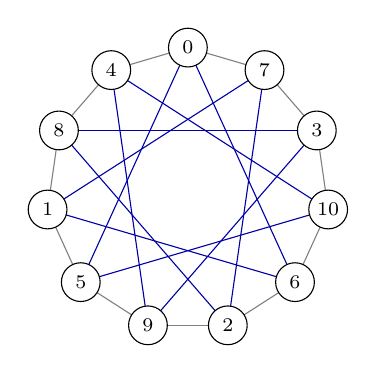
\begin{tikzpicture}[scale=0.90,v/.style={circle,draw,fill=white,inner sep=1pt,minimum size=14pt,font=\scriptsize}]
\draw[gray] (0.0000,2.0000) -- (-1.0813,1.6825);
\draw[blue!65!black] (0.0000,2.0000) -- (-1.5115,-1.3097);
\draw[blue!65!black] (0.0000,2.0000) -- (1.5115,-1.3097);
\draw[gray] (0.0000,2.0000) -- (1.0813,1.6825);
\draw[gray] (-1.9796,-0.2846) -- (-1.5115,-1.3097);
\draw[blue!65!black] (-1.9796,-0.2846) -- (1.5115,-1.3097);
\draw[blue!65!black] (-1.9796,-0.2846) -- (1.0813,1.6825);
\draw[gray] (-1.9796,-0.2846) -- (-1.8193,0.8308);
\draw[gray] (0.5635,-1.9190) -- (1.5115,-1.3097);
\draw[blue!65!black] (0.5635,-1.9190) -- (1.0813,1.6825);
\draw[blue!65!black] (0.5635,-1.9190) -- (-1.8193,0.8308);
\draw[gray] (0.5635,-1.9190) -- (-0.5635,-1.9190);
\draw[gray] (1.8193,0.8308) -- (1.0813,1.6825);
\draw[blue!65!black] (1.8193,0.8308) -- (-1.8193,0.8308);
\draw[blue!65!black] (1.8193,0.8308) -- (-0.5635,-1.9190);
\draw[gray] (1.8193,0.8308) -- (1.9796,-0.2846);
\draw[gray] (-1.0813,1.6825) -- (-1.8193,0.8308);
\draw[blue!65!black] (-1.0813,1.6825) -- (-0.5635,-1.9190);
\draw[blue!65!black] (-1.0813,1.6825) -- (1.9796,-0.2846);
\draw[gray] (-1.5115,-1.3097) -- (-0.5635,-1.9190);
\draw[blue!65!black] (-1.5115,-1.3097) -- (1.9796,-0.2846);
\draw[gray] (1.5115,-1.3097) -- (1.9796,-0.2846);
\node[v] at (0.0000,2.0000) {0};
\node[v] at (-1.0813,1.6825) {4};
\node[v] at (-1.8193,0.8308) {8};
\node[v] at (-1.9796,-0.2846) {1};
\node[v] at (-1.5115,-1.3097) {5};
\node[v] at (-0.5635,-1.9190) {9};
\node[v] at (0.5635,-1.9190) {2};
\node[v] at (1.5115,-1.3097) {6};
\node[v] at (1.9796,-0.2846) {10};
\node[v] at (1.8193,0.8308) {3};
\node[v] at (1.0813,1.6825) {7};
\end{tikzpicture}
% END graph.
\caption{The graph $H$. The outer cycle has vertex order
$0,4,8,1,5,9,2,6,10,3,7$; the other eleven edges are blue chords.}\label{fig:h}
\end{figure}

\section{Proof overview}
The certificate selects pairs of disjoint cycle disks whose total
intersection parity cannot change when the map into $\R^4$ changes.
For one explicit map that parity is odd; for an embedding it would be
zero. The certificate's zero boundary is what makes the parity invariant.

Attach disks along the 46 simple cycles listed in the certificate,
forming a regular cell complex $P$ with one-skeleton $H$.
Appendix~\ref{app:certificate} gives the complete lists.
The certificate also lists 79 unordered pairs of vertex-disjoint disks.
Their sum is a 4-dimensional cycle $\bar z$ in the unordered deleted product
$Q=D(P)/T$, whose cells are unordered pairs of disjoint cells of $P$.
Here $D(P)$ keeps the pairs ordered and $T$ swaps their factors.
Taking both orders gives the symmetric lift $z$ in $D(P)$.
The mod-two intersection cochain on $Q$ evaluates to one on $\bar z$;
equivalently, the cellular invariant $I(z)$ defined in
Section~\ref{sec:obstruction} is one. The obstruction theorem of
van der Holst and Pendavingh then excludes an embedding of $P$ in
$\R^4$. An embedding of the full cycle complex would restrict to one
of $P$, so $H$ is not 4-flat.

The absence of Heawood-family minors follows independently from
$H\subset G_1$ and the minor exclusion in \cite{Graham}.
The two exact minor checks from that paper are repeated by the
accompanying verification.

\section{The deleted-product obstruction}\label{sec:obstruction}
All chains in this section have coefficients in $\F$.
A disk attached along the cycle $(v_0,\ldots,v_{r-1})$ has boundary
\[
\partial\Delta=\sum_{i=0}^{r-1}\{v_i,v_{i+1}\},
\qquad v_r=v_0;
\]
an edge has its two endpoints as boundary, and a vertex has boundary zero.
Different disks have distinct open interiors, even if their boundary
cycles overlap.

For a regular cell complex $P$, its \emph{deleted product} $D(P)$
consists of the product cells $a\times b$ for which the closed cells
$a,b$ are disjoint. In the complexes used here, this is equivalent to
disjointness of their sets of graph vertices. The boundary and the
factor-swapping involution $T$ satisfy
\[
\partial(a\times b)=\partial a\times b+a\times\partial b,
\qquad T(a\times b)=b\times a.
\]
In particular, $T$ acts freely on cells and commutes with $\partial$.
A chain $z$ is \emph{symmetric} if $Tz=z$.
A \emph{half-chain} of a symmetric chain $z$ contains one product cell
from each two-element orbit in its support, so $z=c+Tc$.

An \emph{antipodal} cell complex has a cellular involution taking each
closed cell to a disjoint closed cell. The deleted product with factor
swapping is such a complex.
We use the $\mathbb Z_2$-valued invariant $I$ of symmetric cycles
defined by van der Holst and Pendavingh \cite{vdHP}.
In dimension zero, $I(z)$ is the cardinality modulo two of a half-chain
of $z$. For a symmetric $n$-cycle $z$, $n>0$, and any $n$-chain $c$
with $z=c+Tc$, their recurrence is
\begin{equation}\label{eq:recurrence}
I(z)=I(\partial c).
\end{equation}
This is \cite[Lemma 12]{vdHP}, using the author-manuscript numbering
specified in the bibliography.

The embedding obstruction is \cite[Theorem 18]{vdHP}: for a cell complex
$C$ with a simplicial underlying space, every symmetric $n$-cycle $z$
of $D(C)$ has $I(z)=0$ if and only if there is an even map
$C\to\R^n$. An even map is a general-position map for which each pair
of disjoint cells of complementary dimensions has zero mod-two
intersection number. Only the necessary condition for embedding is used.
An open account of this condition and the equality between the crossing
cocycle evaluated on a cycle and $I$ is \cite[Appendix B.1, pp.\ 25--26]{KT}.

\begin{lemma}\label{lem:obstruction}
Let $P$ be obtained from a finite simple graph by attaching separate
disks along a finite list of simple cycles. If $D(P)$ contains a
symmetric 4-dimensional cycle $z$ with $I(z)=1$, then $P$ does not embed in $\R^4$.
\end{lemma}
\begin{proof}
Give each disk its own interior vertex and cone its boundary edges to
that vertex. This triangulates $P$, including when two disk boundaries
share several edges. The triangulation supplies the underlying-space
hypothesis of \cite[Theorem 18]{vdHP}. An embedding would be an even map and hence
force $I(z)=0$, a contradiction.

The conclusion also rules out a topological embedding $e$.
Indeed, there are finitely many pairs of disjoint closed cells, and
their images under $e$ are disjoint compact sets. The minimum of their
positive separations is positive. A sufficiently close general-position
piecewise linear approximation to $e$ therefore keeps every such pair
disjoint. It would be an even map, again contradicting \cite[Theorem 18]{vdHP}.
\end{proof}

The recurrence also gives a finite way of computing the invariant.
Starting with $z_4=z$, choose a half-chain $c_k$ of $z_k$ and put
$z_{k-1}=\partial c_k$ for $k=4,3,2,1$.
Each new chain is symmetric because
$\partial c_k+T\partial c_k=\partial z_k=0$;
it is a cycle because $\partial^2=0$.
Choose also a half-chain $c_0$ of $z_0$.
Repeated use of \cite[Lemma 12]{vdHP}, in the form
\eqref{eq:recurrence}, gives
\begin{equation}\label{eq:base}
I(z)=|c_0|\pmod2.
\end{equation}


\section{The certificate}\label{sec:certificate}
The proof will use Lemma~\ref{lem:obstruction} by verifying
$\partial z=0$ and $I(z)=1$. The moment-curve calculation gives a second
evaluation of the same invariant.
The certificate specifies the edges of $H$, 46 simple cycles
$C_0,\ldots,C_{45}$, and a set $S$ of 79 distinct unordered pairs of
indices. Write $\Delta_i$ for the disk attached along $C_i$, and define
\[
z=\sum_{\{i,j\}\in S}
(\Delta_i\times \Delta_j+\Delta_j\times \Delta_i).
\]
For every pair in $S$, the cycles $C_i,C_j$ are vertex-disjoint.
For every edge $e$ and disk $\Delta_j$, the number of selected pairs
$\{i,j\}$ for which $e$ belongs to $C_i$ is even.
These finite assertions are checked directly and give $\partial z=0$:
they are exactly the coefficients of the edge--disk product cells.

Let $\bar z=\sum_{\{i,j\}\in S}[\Delta_i\times \Delta_j]$ in
$Q=D(P)/T$. The same boundary calculation gives $\partial\bar z=0$;
$z$ is its symmetric lift.

For a general-position map $f:P\to\R^4$, let $\theta_f$ assign to
an unordered pair of disjoint disks the parity of their intersections.
This is a degree-four cochain on $Q$. Changing $f$ changes
$\theta_f$ by a coboundary: intersection tracks in a generic homotopy
give the corresponding degree-three cochain. This is the mod-two
van Kampen obstruction construction; see \cite[Appendix D]{MTW} and
its cellular formulation in \cite[Appendix B.1]{KT}. Consequently
$\langle\theta_f,\bar z\rangle$ is independent of $f$, since
$\partial\bar z=0$. Its value one certifies a nonzero obstruction
class in $H^4(Q;\F)$. An embedding has zero intersections and would
force this pairing to vanish. The equality of this pairing with $I(z)$
is stated explicitly in \cite[Appendix B.1, p.\ 26]{KT}, following
\cite{vdHP}.

There are two independent evaluations of $I(z)$. The cellular
evaluation constructs the ordered chain $z$ and applies
\eqref{eq:recurrence} down through dimensions four, three, two and one.
At every dimension it checks symmetry and zero boundary before choosing
one cell from each swapping orbit. Equation~\eqref{eq:base} gives one.

For the intersection evaluation, triangulate each $\Delta_i$ by coning its
boundary to its private center. Place graph vertex $v$ at parameter
$t=v$ and center $i$ at parameter $t=11+i$ on the moment curve
\[
m(t)=(t,t^2,t^3,t^4).
\]
Extend linearly over each triangle.
Two triangles with disjoint vertex sets meet precisely when their six
parameters, in increasing order, alternate between the triangles.
Indeed, every five moment-curve points are affinely independent,
and the unique affine dependence of six such points has alternating
coefficient signs, by the Vandermonde determinant. Its two sign classes
form the Radon partition, giving a single transverse intersection
exactly in the alternating case. This is the standard moment-curve
test; see \cite[Lemma D.2]{MTW}. A triangle and a disjoint edge cannot
meet, again by affine independence of five points.
A sufficiently small general-position perturbation therefore preserves
these intersection parities.

For each unordered disk pair in $S$, sum this alternating-order test
over its pairs of cone triangles, and then sum over $S$, modulo two.
The pairing identity above identifies the resulting bit with $I(z)$.
This second computation also gives one. Both evaluations use integer and mod-two operations;
neither involves a floating-point approximation.

\begin{proof}[Proof of Theorem~\ref{thm:main}]
The finite checks above establish that $z$ is a symmetric 4-dimensional cycle
with $I(z)=1$. Lemma~\ref{lem:obstruction} excludes an embedding of $P$.
Since $P$ is a subcomplex of the full cycle complex of $H$, the graph
$H$ is not 4-flat.

The edge list identifies $H$ exactly with $G_1-\{1,10\}$ in
\cite{Graham}. That paper's Theorem~1, also checked by the accompanying
minor computations, excludes every Heawood-family minor of $G_1$.
Every minor of $H$ is a minor of $G_1$, so $H$ has no such minor.

Finally, 4-flat graphs form a minor-closed class
\cite[\S1.1]{GW}, following van der Holst \cite{vdH}. Choose a minor of $H$ minimal among its non-4-flat
minors; this is possible because a finite graph has finitely many
minors up to isomorphism. It is an excluded minor for 4-flatness and
cannot belong to the Heawood family, completing the proof.
\end{proof}

\section{Computational verification}
The accompanying data and Appendix~\ref{app:certificate} give the cycles
and disk pairs explicitly.
Each of the two separately written checkers validates the graph,
the simplicity of each cycle, the disjointness of each selected pair
and the boundary condition. Both read the same graph, cycle list and
selected pairs from the JSON
certificate. Checker A alone fan-triangulates the disks with private
centers and evaluates moment-curve intersections; checker B keeps the
disks unsplit and uses their cellular boundaries in the recurrence.
The implementations share no checking code.
Both accept the certificate for $H$, as well as certificates for
$G_1$ and the known non-4-flat graph $K_7$.
For each of $H$ and $G_1$, removing the final listed disk pair gives
a nonzero boundary and is rejected by both checkers. A second negative
control takes two disjoint copies of the $K_7$ certificate. Its nonzero
chain has zero boundary and invariant $1+1=0$, so both checkers must
reject it at the parity test.
The proof needs only the listed subcomplex; completeness of the cycle
list is irrelevant.

The minor exclusion uses the two independent implementations published
with \cite{Graham}. One enumerates edge deletions and contractions and
tests isomorphism against the Heawood family; the other searches for
branch sets. Since $G_1$ has 23 edges and every Heawood graph has 21 or
22, at most two edge operations can lead to a Heawood minor.
Vertex deletions are covered by deleting incident edges and removing
isolated vertices. The family is regenerated by closing $K_7$ and
$K_{3,3,1,1}$ under the stated transformations, giving 20 graphs with
21 edges and 58 with 22 edges, as recorded in \cite[\S2]{MPi}.
The implementations also detect Heawood minors in the supplied
positive examples. The public check also makes all 45 direct comparisons:
$H$ itself and its 22 single-edge deletions and 22 single-edge contractions. A minor requiring at least two edge
operations has at most 20 edges, fewer than any Heawood graph.
For each of the 44 proper minors, it also finds a pair of vertices whose
deletion leaves a planar graph, independently verifying the proper-minor
input to Corollary~\ref{cor:minimal}.

The complete verification takes less than a minute on one CPU core.
The accompanying README gives the dependencies and reproduction
command. The finite certificates and their arithmetic are checked
by these programs; the topological implication relies on the two
cited inputs from van der Holst and Pendavingh and their intersection
interpretation, also presented in \cite[Appendix B]{KT}. The proof is not formalized in a proof assistant.

% BEGIN generated certificate appendix
\begin{appendices}
\section{The explicit certificate}\label{app:certificate}
The following lists completely specify the subcomplex $P$ and the cycle
$\bar z=\sum_{(i,j)\in S}[\Delta_i\times \Delta_j]$ in the unordered deleted product.
A row $(v_0,\ldots,v_r)$ denotes the closed cycle with successive edges
$v_0v_1,\ldots,v_{r-1}v_r,v_rv_0$. All indices start at zero.
\begin{center}\small
\begin{tabular}{r l @{\qquad} r l}
$i$ & $C_i$ & $i$ & $C_i$\\\hline
0 & $(0,4,8,1,5)$ & 23 & $(1,5,9,3,7)$\\
1 & $(0,4,8,1,7)$ & 24 & $(1,5,9,4,8)$\\
2 & $(0,4,8,2,6)$ & 25 & $(1,5,10,3,7)$\\
3 & $(0,4,8,3,7)$ & 26 & $(1,5,10,3,8)$\\
4 & $(0,4,9,2,6)$ & 27 & $(1,5,10,6)$\\
5 & $(0,4,9,2,7)$ & 28 & $(1,6,2,7)$\\
6 & $(0,4,9,3,10,5)$ & 29 & $(1,6,2,8)$\\
7 & $(0,4,9,5)$ & 30 & $(1,6,10,3,8)$\\
8 & $(0,4,10,3,7)$ & 31 & $(1,6,10,4,8)$\\
9 & $(0,4,10,3,9,5)$ & 32 & $(1,7,2,8)$\\
10 & $(0,4,10,5)$ & 33 & $(1,7,3,8)$\\
11 & $(0,4,10,5,1,6)$ & 34 & $(2,6,10,3,7)$\\
12 & $(0,4,10,6)$ & 35 & $(2,6,10,3,9)$\\
13 & $(0,5,1,6)$ & 36 & $(2,6,10,4,8)$\\
14 & $(0,5,1,7)$ & 37 & $(2,6,10,5,9)$\\
15 & $(0,5,9,2,7)$ & 38 & $(2,7,3,8)$\\
16 & $(0,5,9,3,7)$ & 39 & $(2,7,3,8,4,9)$\\
17 & $(0,5,10,6)$ & 40 & $(2,7,3,9)$\\
18 & $(0,6,1,7)$ & 41 & $(2,8,3,9)$\\
19 & $(0,6,2,7)$ & 42 & $(2,8,4,9)$\\
20 & $(0,6,10,3,7)$ & 43 & $(3,8,4,9,5,10)$\\
21 & $(1,5,9,2,6)$ & 44 & $(3,8,4,10)$\\
22 & $(1,5,9,2,8)$ & 45 & $(3,9,5,10)$\\
\end{tabular}\end{center}
For every graph edge $e$ and every disk index $j$, count the selected
pairs containing $j$ whose other cycle contains $e$. These are the
coefficients of $\partial\bar z$; every count is even. The nonzero
integer counts have the following multiplicities: 2 occurs 340 times, 4 occurs 12 times.
Thus $\partial\bar z=0$; equivalently the ordered lift $z$ is a cycle.
\par The table below lists every pair in $S$ and its moment-curve
intersection coefficient $\theta_{ij}$. For a direct check, cone $C_i$
to parameter $11+i$ and order each six-element set of two disjoint
triangles. A triangle pair contributes one exactly when its two
triples alternate in that order. Sum these contributions for each
disk pair and reduce modulo two.
\begin{center}\small
\begin{tabular}{r r r @{\qquad} r r r @{\qquad} r r r}
$i$&$j$&$\theta_{ij}$&$i$&$j$&$\theta_{ij}$&$i$&$j$&$\theta_{ij}$\\\hline
0 & 34 & 1 & 8 & 22 & 1 & 16 & 36 & 0\\
0 & 35 & 1 & 8 & 29 & 0 & 17 & 32 & 0\\
0 & 40 & 0 & 9 & 28 & 0 & 17 & 33 & 0\\
1 & 35 & 1 & 9 & 29 & 0 & 17 & 39 & 0\\
1 & 37 & 1 & 9 & 32 & 0 & 17 & 42 & 0\\
1 & 45 & 0 & 10 & 38 & 0 & 18 & 41 & 0\\
2 & 23 & 0 & 10 & 40 & 0 & 18 & 42 & 0\\
2 & 25 & 0 & 10 & 41 & 0 & 18 & 43 & 0\\
2 & 45 & 0 & 11 & 38 & 0 & 18 & 45 & 0\\
3 & 21 & 1 & 11 & 40 & 0 & 19 & 24 & 0\\
3 & 27 & 0 & 11 & 41 & 0 & 19 & 26 & 0\\
3 & 37 & 1 & 12 & 22 & 0 & 19 & 43 & 0\\
4 & 25 & 0 & 12 & 23 & 0 & 20 & 22 & 1\\
4 & 26 & 0 & 12 & 32 & 0 & 20 & 24 & 1\\
4 & 33 & 0 & 12 & 40 & 0 & 20 & 42 & 0\\
5 & 26 & 0 & 13 & 38 & 0 & 21 & 44 & 0\\
5 & 27 & 0 & 13 & 39 & 0 & 23 & 36 & 0\\
5 & 30 & 0 & 13 & 42 & 0 & 24 & 34 & 1\\
6 & 28 & 0 & 14 & 35 & 0 & 25 & 42 & 0\\
6 & 29 & 0 & 14 & 36 & 0 & 27 & 39 & 0\\
6 & 32 & 0 & 14 & 41 & 0 & 28 & 43 & 0\\
7 & 29 & 0 & 14 & 44 & 0 & 28 & 44 & 0\\
7 & 30 & 0 & 15 & 30 & 0 & 29 & 45 & 0\\
7 & 32 & 0 & 15 & 31 & 0 & 31 & 40 & 0\\
7 & 33 & 0 & 15 & 44 & 0 & 33 & 37 & 0\\
7 & 34 & 0 & 16 & 29 & 0 &  &  & \\
8 & 21 & 1 & 16 & 31 & 0 &  &  & \\
\end{tabular}\end{center}
Exactly 11 of the 79 listed coefficients are one. Hence
$\langle\theta,\bar z\rangle=1$ in $\mathbf F_2$. The ordered-lift
half-chain calculation independently gives $I(z)=1$.
The public check regenerates this appendix from \texttt{data/h.json}
and requires an exact match; both obstruction checkers independently
verify the underlying certificate.
\end{appendices}
% END generated certificate appendix

\begin{thebibliography}{10}
\bibitem{GW}
A. Georgakopoulos and M. Winter,
On 2-complexes embeddable in 4-space, and the excluded minors of their
underlying graphs,
\href{https://arxiv.org/abs/2408.12681v1}{arXiv:2408.12681v1} (2024).

\bibitem{Graham}
P. Graham,
The Heawood family is not the complete list of excluded minors for
Colin de Verdi\`ere invariant at most 5,
\emph{heawood-family-mu5}, version 1 (2026),
\href{https://doi.org/10.5281/zenodo.24128771}
{doi:10.5281/zenodo.24128771}.

\bibitem{KM}
H. Kim and T. W. Mattman,
Dips at small sizes for topological graph obstruction sets,
\emph{Discrete Appl. Math.} 360 (2025), 139--166,
\href{https://doi.org/10.1016/j.dam.2024.08.022}
{doi:10.1016/j.dam.2024.08.022}.
Section numbers refer to
\href{https://arxiv.org/abs/2205.14255v2}{arXiv:2205.14255v2}.

\bibitem{MP}
T. W. Mattman and A. Pavelescu,
Three thousand obstructions to knotless embedding,
\href{https://arxiv.org/abs/2607.01414v1}{arXiv:2607.01414v1} (2026).

\bibitem{MPi}
T. W. Mattman and M. Pierce,
The $K_{n+5}$ and $K_{3^2,1^n}$ families and obstructions to $n$-apex,
in \emph{Knots, Links, Spatial Graphs, and Algebraic Invariants},
Contemp. Math. 689, Amer. Math. Soc., 2017, 137--158,
\href{https://doi.org/10.1090/conm/689/13856}
{doi:10.1090/conm/689/13856}.
Section numbers refer to
\href{https://arxiv.org/abs/1603.00885v1}{arXiv:1603.00885v1}.

\bibitem{KT}
V. Kalu\v{z}a and M. Tancer,
Even maps, the Colin de Verdi\`ere number and representations of graphs,
\href{https://arxiv.org/abs/1907.05055v2}{arXiv:1907.05055v2} (2020).
All page and proposition references use this version.

\bibitem{MTW}
J. Matou\v{s}ek, M. Tancer and U. Wagner,
Hardness of embedding simplicial complexes in $\R^d$,
\emph{J. Eur. Math. Soc.} 13 (2011), 259--295,
\href{https://doi.org/10.4171/JEMS/252}{doi:10.4171/JEMS/252}.

\bibitem{vdHLS}
H. van der Holst, L. Lov\'asz and A. Schrijver,
The Colin de Verdi\`ere graph parameter,
in \emph{Graph Theory and Combinatorial Biology},
Bolyai Soc. Math. Stud. 7 (1999), 29--85,
\href{https://ir.cwi.nl/pub/1257/1257D.pdf}{open text}.

\bibitem{vdH}
H. van der Holst,
Graphs and obstructions in four dimensions,
\emph{J. Combin. Theory Ser. B} 96 (2006), 388--404,
\href{https://doi.org/10.1016/j.jctb.2005.09.004}
{doi:10.1016/j.jctb.2005.09.004}.

\bibitem{vdHP}
H. van der Holst and R. A. Pendavingh,
On a graph property generalizing planarity and flatness,
\emph{Combinatorica} 29 (2009), 337--361,
\href{https://doi.org/10.1007/s00493-009-2219-6}
{doi:10.1007/s00493-009-2219-6}.
Lemma~12, Theorem~18 and section numbers refer to the
\href{https://www.researchgate.net/publication/220441340_On_a_graph_property_generalizing_planarity_and_flatness}
{author manuscript dated April 26, 2008}.
\end{thebibliography}
\end{document}
